\subsubsection{User scenarios}
\subsubsection*{Scenario 3}
Jishnu, a Telengana’s farmer, finds out about Dream forum and wants to read some posts. He clicks on the link found using a browser and selects his region, finding out the last review document published by a Policy maker. Once he has read the discussion he decides to make his contribution and shares the agricultural techniques he uses.
Jishnu hasn’t got an account yet, but he needs to be registered to post on the forum. For this purpose, he clicks on the “Sign up” button on the top right and he inserts his data in the following page, including the region in which he lives, his personal email address and eventually he chooses a safe password to protect his new account. Once he clicks on the confirmation button, the system tells him to check the email he has used to register to conclude the registration process. He opens his mail looking for a mail from Dream containing a confirmation link. When he clicks on it a browser page pops up containing a check message which confirms that the registration ended correctly. Now he can login from the home page, go to the page he was visiting and add his comment.

\subsubsection*{Scenario 4}
Basant is an active User of the forum of the site Dream. Unluckily, he discovers that the last post he published on a discussion contains a file that is not the file he wants to publish. So he returns to that post, clicks on the modify button and replaces the file with the correct one. After doing this procedure he clicks the confirmation button and then the changes to his post go to the pending approval list of the system.

\subsubsection*{Use case diagram}
\begin{figure}[h!]
        \centering
        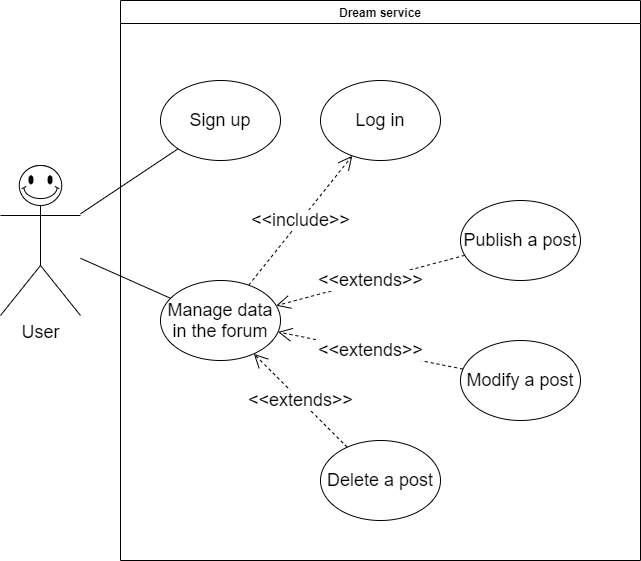
\includegraphics[scale=0.40]{images/use_cases_diagram/user_use_case.png}
        \caption{Use case diagram}
        \label{fig:user_use_case}
    \end{figure}
    
    \newpage
    
\subsubsection*{Use case tables}

\begin{longtable}{p{.25\textwidth} | p{.75\textwidth}}
 \caption{Sign Up User}
    \label{tab:sign_up}\\
        \hline
        \textbf{ID} & 4\\
        \hline
        \textbf{Name}  &  Sign up User\\
        \hline
        \textbf{Actor}  &  User\\
        \hline
        \textbf{Entry condition}  &  User has reached the site\\
        \hline
        \textbf{Input} & Personal data,
        email and password to use for the registration\\
        \hline
        \textbf{Events flow} & \begin{itemize}
                \item The site displays the “Sign up” button on the top right of the screen
                \item User clicks on “Sign up”
                \item The site displays a new page containing blank fields where user has to insert his data: name, surname, date of birth, area of residence, email and password
                \item User inserts the mandatory data and accepts the “Terms of Service”
                \item User confirms by clicking the confirmation button
                \item The page shows a message inviting User to visit his email address in order to conclude the registration
                \item User opens his inbox, find the email from Dream and clicks on confirmation link
                \item The site displays a confirmation message of successful registration
                \end{itemize}
                 \\
        \hline
        \textbf{Exit condition} & User registration has been successful: the inserted data are stored in the database of the system. Now User can login using his credentials and post in the forum\\
        \hline
        \textbf{Output} & Registration data are stored in the database of Dream site.\\
        \hline
        \textbf{Exception} & \begin{itemize}
            \item User inserts non valid data(e.g. wrong email format or nonexistent area). The application displays an error message telling the User that he must check the data inserted and correct the invalid ones
            \item User inserts an e-mail which is already stored in the in the database. So, after user inserts his data and clicks on confirm, the application displays an error message telling User that he’s already registered to the service and invites him to login with that email
    \end{itemize} \\\hline
   
    \end{longtable}
     
     \begin{figure}[h!]
        \centering
        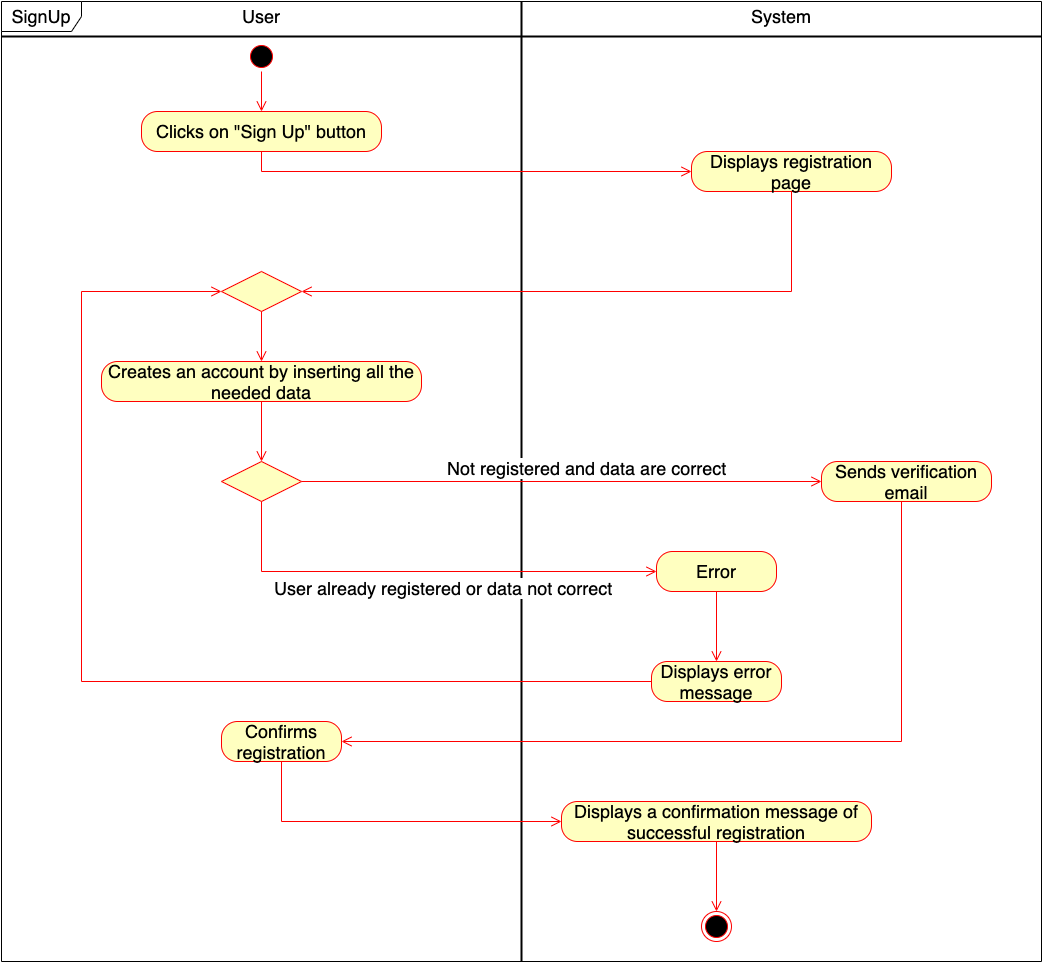
\includegraphics[scale=0.35]{images/use_cases_diagram/user_sign_up.png}
        \caption{Sign Up  User}
        \label{fig:usr_sign_up}
    \end{figure}
     \FloatBarrier
     
    \begin{longtable}{p{.25\textwidth} | p{.75\textwidth}}
     \caption{Login User}
        \label{tab:login_user}\\
        \hline
        \textbf{ID} & 5\\
        \hline
        \textbf{Name}  &  Login User\\
        \hline
        \textbf{Actor}  &  User\\
        \hline
        \textbf{Entry condition}  &  
        \begin{itemize}
                \item User has reached the site
                \item User is already registered to the platform
         \end{itemize}\\
        \hline
        \textbf{Input} & User email and password associated to a successful registration\\
        \hline
        \textbf{Events flow} & 
        \begin{itemize}
                \item The site displays the “Sign In” button on the top right of the screen
                \item User clicks on “Sign In”
                \item The system displays the login page
                \item User fills the username (email) and password fields using the credential inserted during the registration
                \item System checks the validity of the credentials inserted
                \item The system displays the precedent page or, if unavailable, the home page of the site
                 \end{itemize}
                 \\
        \hline
        \textbf{Exit condition} & User is logged in\\
        \hline
        \textbf{Exceptions} & User inserts wrong credentials and clicks on “login” button. The system shows an error message inviting the User to check the credentials before trying again to login\\
        \hline
       
    \end{longtable}
    \begin{figure}[h!]
        \centering
        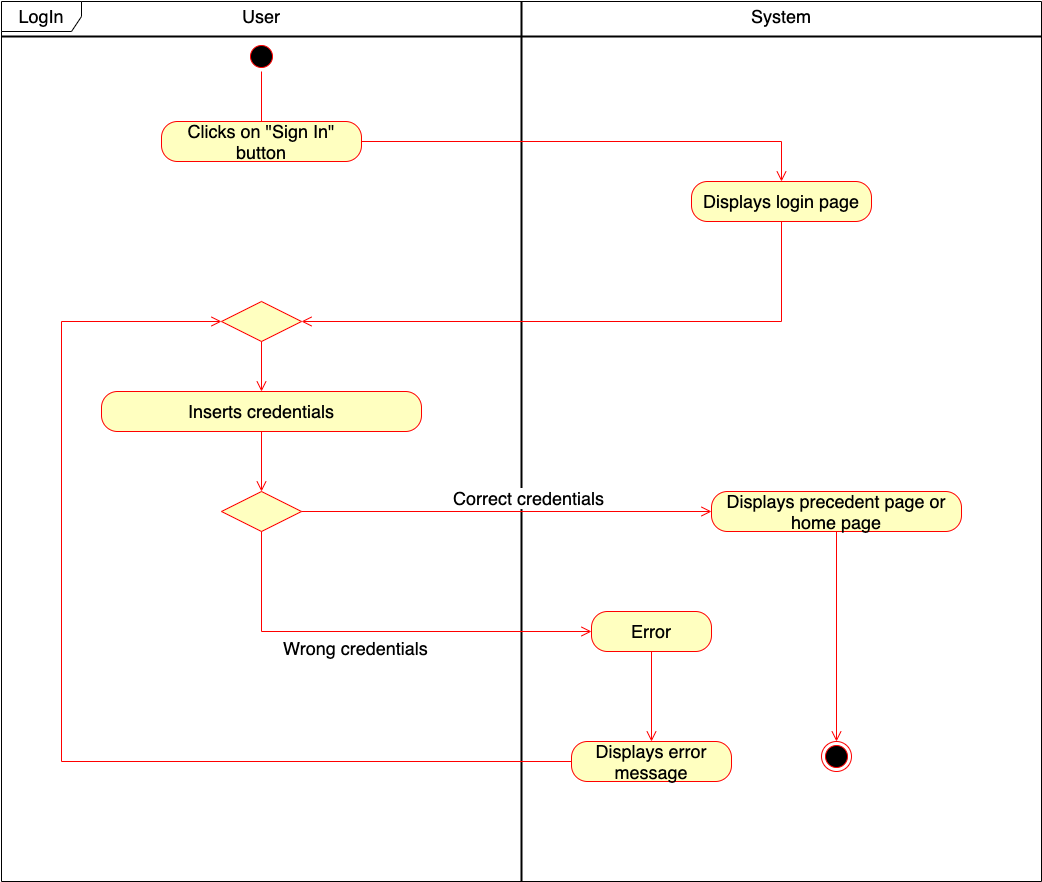
\includegraphics[scale=0.35]{images/use_cases_diagram/user_login.png}
        \caption{Login User}
        \label{fig:user_login}
    \end{figure}
    \FloatBarrier
    
    \begin{longtable}{p{.25\textwidth} | p{.75\textwidth}}
    \caption{Publish a post by User}
        \label{tab:publish_post_by_user}\\
        \hline
        \textbf{ID} & 6\\
        \hline
        \textbf{Name}  &  Publish a post by User\\
        \hline
        \textbf{Actor}  &  User\\
        \hline
        \textbf{Entry condition}  &  
        \begin{itemize}
                \item The User is already registered in the system
                \item The User is already logged in the system
                \item The User is in the forum home page
         \end{itemize}\\
        \hline
        \textbf{Input} & Post\\
        \hline
        \textbf{Events flow} & 
        \begin{itemize}
                \item The User selects the section of his interest
                \item The User selects the discussion about the argument of interest
                \item The User inserts a new answer in the form
                \item The User confirms the answer by clicking the confirmation button
                 \end{itemize}
                 \\
        \hline
        \textbf{Exit condition} & The answer is in pending approval\\
        \hline
        \textbf{Exceptions} & The User tries to insert invalid contents (invalid characters, invalid file format, etc...)\\
        \hline
        
    \end{longtable}
    
    \begin{figure}[h!]
        \centering
        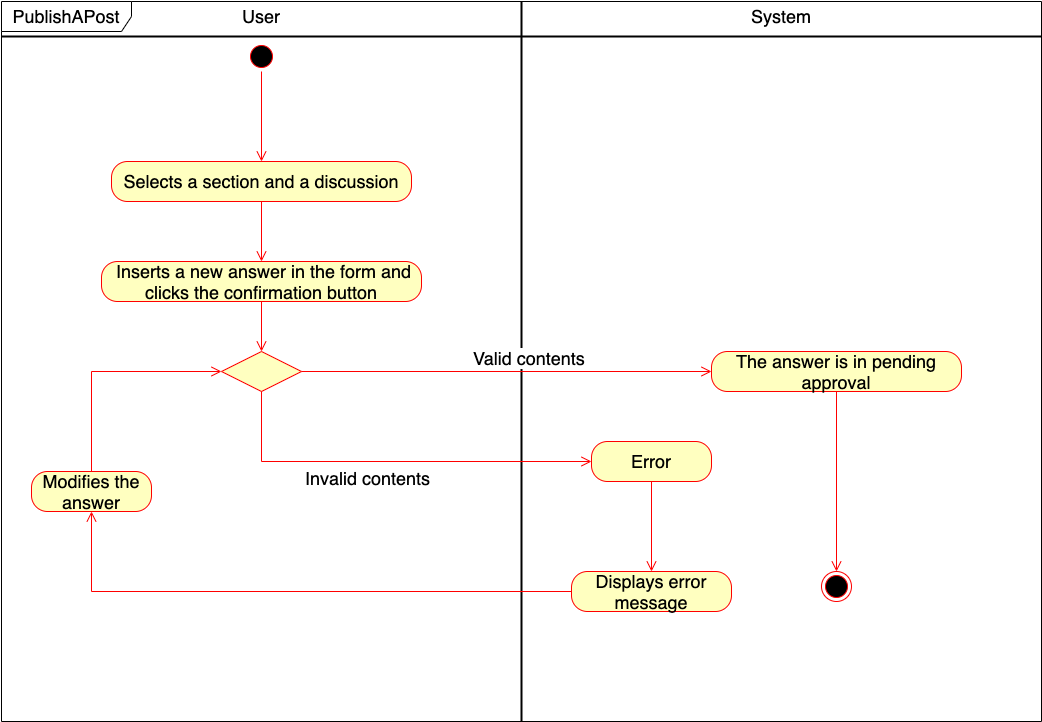
\includegraphics[scale=0.35]{images/use_cases_diagram/user_publish_post.png}
        \caption{Publish a post by User}
        \label{fig:publish_post_by_user}
    \end{figure}
   \newpage
    \begin{longtable}{p{.25\textwidth} | p{.75\textwidth}}
    \caption{Modify a post by User}
        \label{tab:modify_post_by_user}\\
        \hline
        \textbf{ID} & 7\\
        \hline
        \textbf{Name}  &  Modify a post by User\\
        \hline
        \textbf{Actor}  &  User\\
        \hline
        \textbf{Entry condition}  &  
        \begin{itemize}
                \item The User is already registered in the system
                \item The User is already logged in the system
                \item The User is in the discussion page where the post is present
                \item The User has already published the post
         \end{itemize}\\
        \hline
        \textbf{Input} & Post\\
        \hline
        \textbf{Events flow} & 
        \begin{itemize}
                \item The User press on the “Modify” button on the selected post
                \item The System returns to the User the edit page
                \item The User introduces the changes in the post
                \item The User confirms the changes by clicking the confirmation button

                 \end{itemize}
                 \\
        \hline
        \textbf{Exit condition} & The changes to the post are visible\\
        \hline
        \textbf{Exceptions} &  The User  tries to insert invalid contents (invalid characters, invalid file format, etc...)\\
        \hline
        \textbf{Special requirements} & The User can modify only post written by his account \\ \hline
        
    \end{longtable}
    \begin{figure}[h!]
        \centering
        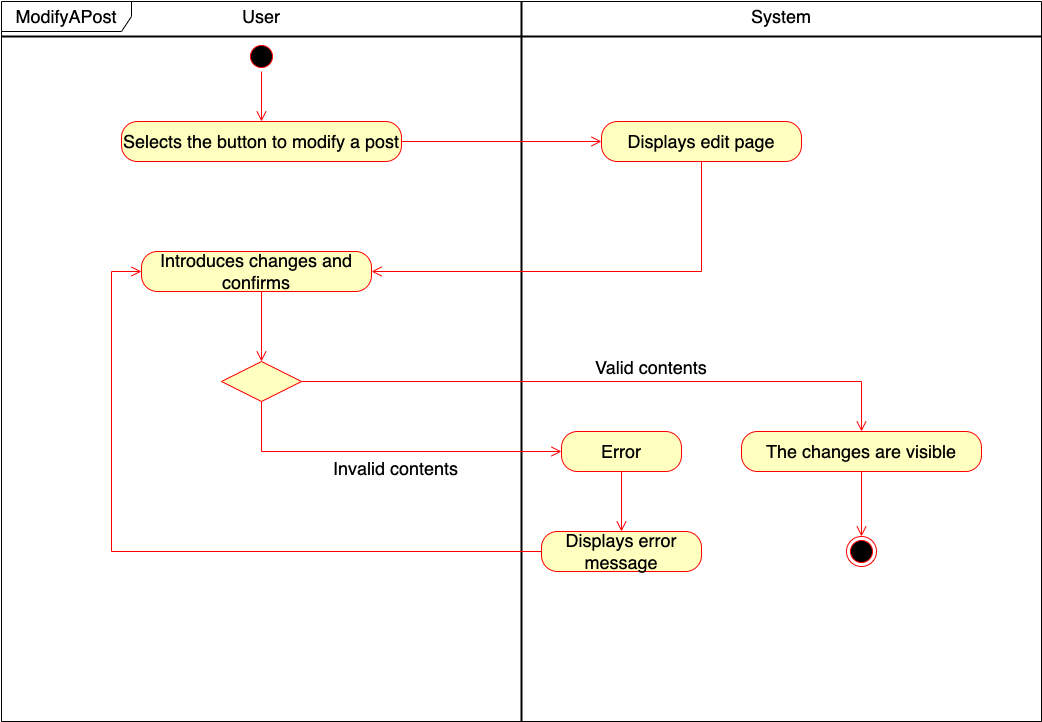
\includegraphics[scale=0.35]{images/use_cases_diagram/user_modify_post.png}
        \caption{Modify a post by User}
        \label{fig:user_modify_post}
    \end{figure}
    \FloatBarrier
    
                \begin{longtable}{p{.25\textwidth} | p{.75\textwidth}}
        \caption{Delete a post by User}
    \label{tab:user_delete_post}\\
        \hline
        \textbf{ID} & 8\\
        \hline
        \textbf{Name}  &  Delete post by User\\
        \hline
        \textbf{Actor}  &  User\\
        \hline
        \textbf{Entry condition}  &  \begin{itemize}
            \item  The User is already registered in the system
            \item  The User is already logged in the system
            \item  The User is in the discussion page where the post is present
            \item The User has already published the post
        \end{itemize}\\
        \hline
        \textbf{Input} & Post\\
        \hline
        \textbf{Events flow} & \begin{itemize}
                \item The User press on the “Delete” button on the selected post
                \item The System returns to the User a confirmation message
                \item The User confirms the operation by clicking the confirmation button
                \end{itemize}
                 \\
        \hline
        \textbf{Exit condition} & The post is deleted from the forum\\
        \hline
        \textbf{Exception} & The User doesn't confirm the operation\\ \hline
        \textbf{Special requirements} & The User can delete only post written by his account \\ \hline

    
    \end{longtable}
      \begin{figure}[h!]
        \centering
        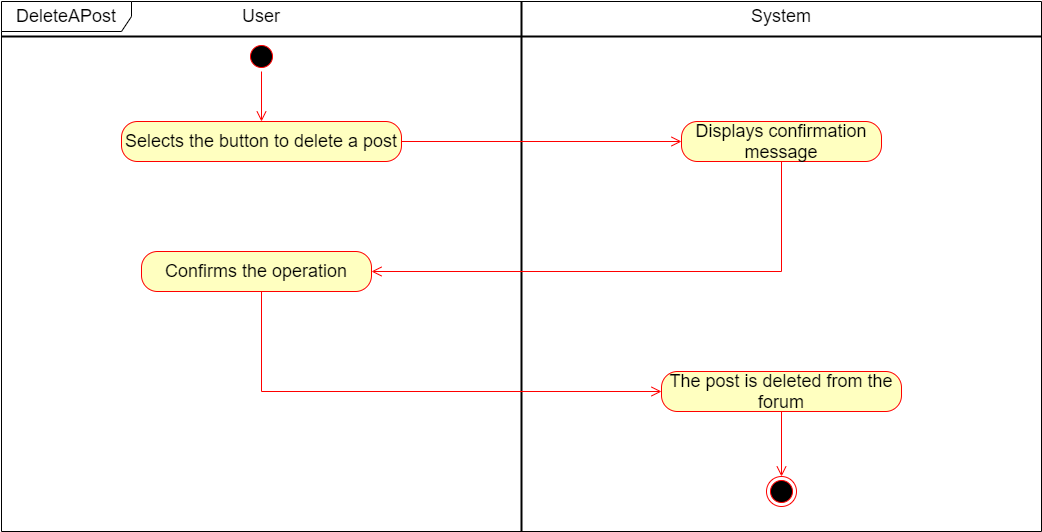
\includegraphics[scale=0.35]{images/use_cases_diagram/user_delete_post.png}
        \caption{Delete a post by User}
        \label{fig:user_delete_post}
    \end{figure}
    \FloatBarrier